% +------------------------------------------------------------------------+
% | Skin_surface_3/doc_tex/Skin_surface_3/main.tex
% +------------------------------------------------------------------------+
% | Meshing the 3d Skin surface defined for a set of spheres.
% | 
\RCSdef{\skinSurfaceRev}{$Id$}
\RCSdefDate{\skinSurfaceDate}{$Date$}
% +------------------------------------------------------------------------+

\chapter{3D Skin Surface Meshing}
\label{chapterSkinSurface}
\ccChapterRelease{\skinSurfaceRev. \ \skinSurfaceDate}
\ccChapterAuthor{Nico Kruithof}

\minitoc

% +------------------------------------------------------------------------+
\section{Introduction}
\label{sectionSkinSurfaceIntro}

Skin surfaces, introduced by Edelsbrunner in \cite{cgal:e-dssd-99},
have a rich and simple combinatorial and geometric structure that
makes them suitable for modeling large molecules in biological
computing.  Meshing such surfaces is often required for further
processing of their geometry, like in numerical simulation and
visualization.

A skin surface is parameterized by a set of weighted points (input
balls) and a shrink factor. If the shrink factor is equal to one, the
surface is just the boundary of the union of the input balls.  If the
shrink factor decreases, the skin surface becomes tangent continuous,
due to the appearance of patches of spheres and hyperboloids
connecting the balls.

This package constructs an isotopic mesh from a set of balls and a
shrink factor using the algorithm described in
\cite{cgal:kv-mssct-05}. An optimized algorithm is implemented for
meshing the union of a set of balls.

\section{Definition}
A skin surface is defined as the boundary of an infinite set of balls.
Let $\mathcal{P}$ be a set of weighted points in $\R^3$. A weighted
point ${\hat{p}}=(p,w_p)$ can also be seen as a ball with center $p$
and squared radius $w_p$. A vector space of weighted points is
inherited from the bijective map
\[\Pi({\hat{p}}) = ({p, \|{p}\|^2-w_p})\]
where $\|{p}\|$ is the two-norm. Addition of two weighted points and
the multiplication of a weighted point by a scalar are defined in the
vector space structure inherited under $\Pi$.

A shrunk weighted point ${\hat{p}}^{s}$ is obtained by multiplying the
weight of the weighted point ${\hat{p}}$ with the scalar $s$:
${\hat{p}}^{s}= (p,s w_p)$. A set of weighted points is shrunk by
shrinking each weighted point seperately.

The skin surface of ${\mathcal{P}}$ with shrink factor $s$ is the boundary
of the weighted points in the convex hull of $\mathcal{P}$ shrunk by a
factor $s$:
\[{\tt skn}^s(\mathcal{P}) =
\partial({\tt conv}(\mathcal{P}))^s\]

A polyhedral complex called the mixed complex subdivides the skin
surface into quadric patches (spheres and hyperboloids). A mixed cell
exists for every simplex in the Regular triangulation. Adding alpha to
the weight of each weighted point in $\mathcal{P}$, does not change the
mixed complex. For a shrink factor of one, the mixed complex
degenerates into the Voronoi diagram.

\section{Skin surface mesh}
The mesh is constructed in several steps:
\begin{enumerate}
\item Triangulate the mixed complex
\item Extract the mesh from the constructed triangulation
\item Apply modifications to the mesh
\end{enumerate}
Each of these steps is of independent interest and we describe them in
more detail.

\subsection{Triangulation of the mixed complex.}
The construction of the triangulated mixed complex uses a
\ccc{Triangulation_incremental_builder_3} that constructs a
triangulation from vertices and cells. This builder first gets the
vertices of the triangulation and then the cells, which are defined by
references to four vertices. From these vertices and cells it
constructs the triangulation.

The function \ccc{triangulate_mixed_complex_3} computes the vertices
and cells of the triangulation and inserts them in the
\ccc{Triangulation_incremental_builder_3}. The construction of
vertices is complicated due to the occurrence of many degenerate
cases.  For example, let $\nu_{\mathcal{X}}$ be a Voronoi edge and
let $\nu{\mathcal{X}'}, \nu{\mathcal{X}''}$ be its two vertices.
If the Voronoi edge degenerates into a point, then the anchor points
$a_{f({\mathcal{X}})}{\nu{\mathcal{X}}}$,
$a_{f({\mathcal{X}})}{\nu{\mathcal{X}'}}$ and
$a_{f({\mathcal{X}})}{\nu{\mathcal{X}''}}$ are equal. Similar
cases occur if a Voronoi facet degenerates into a line segment or a
Voronoi cell into a facet. We first compute the anchor points of the
triangulated mixed complex and combine anchor points that are equal
using a union-find datastructure. We then insert all unique vertices
and the tetrahedra that are not degenerate, i.e., have four distinct
vertices.

\subsubsection{Union of balls}
For the boundary of the union of a set of balls, it is not necessary
to triangulate all mixed cells since the only non-degenerate cells are
mixed cells corresponding to Voronoi cells. For efficient meshing of
the boundary of a union of balls we implemented a function
\ccc{triangulate_voronoi_diagram_3} that is similar to
\ccc{triangulate_mixed_complex_3}.



\subsection{Marching tetrahedra}
The marching tetrahedra algorithm, introduced in
\cite{cgal:tpg-rmtiise-99}, extracts a surface from a triangulation.
First, it labels each vertex of the triangulation either as inside or
as outside. Using these labels the vertices of the mesh are
constructed as the intersection point of the surface and an edge with
different vertex-labels. The faces of the mesh are defined by the
tetrahedra of the triangulation. Based on the number of
triangulation-vertices inside the surface, we can distinguish five
cases, two of which are redundant if we allow the exchange of inside
and outside. These three cases are depicted in
Figure~\ref{SkinSurface3-fig-marching}.

\begin{figure}
\begin{ccTexOnly}
\begin{center}
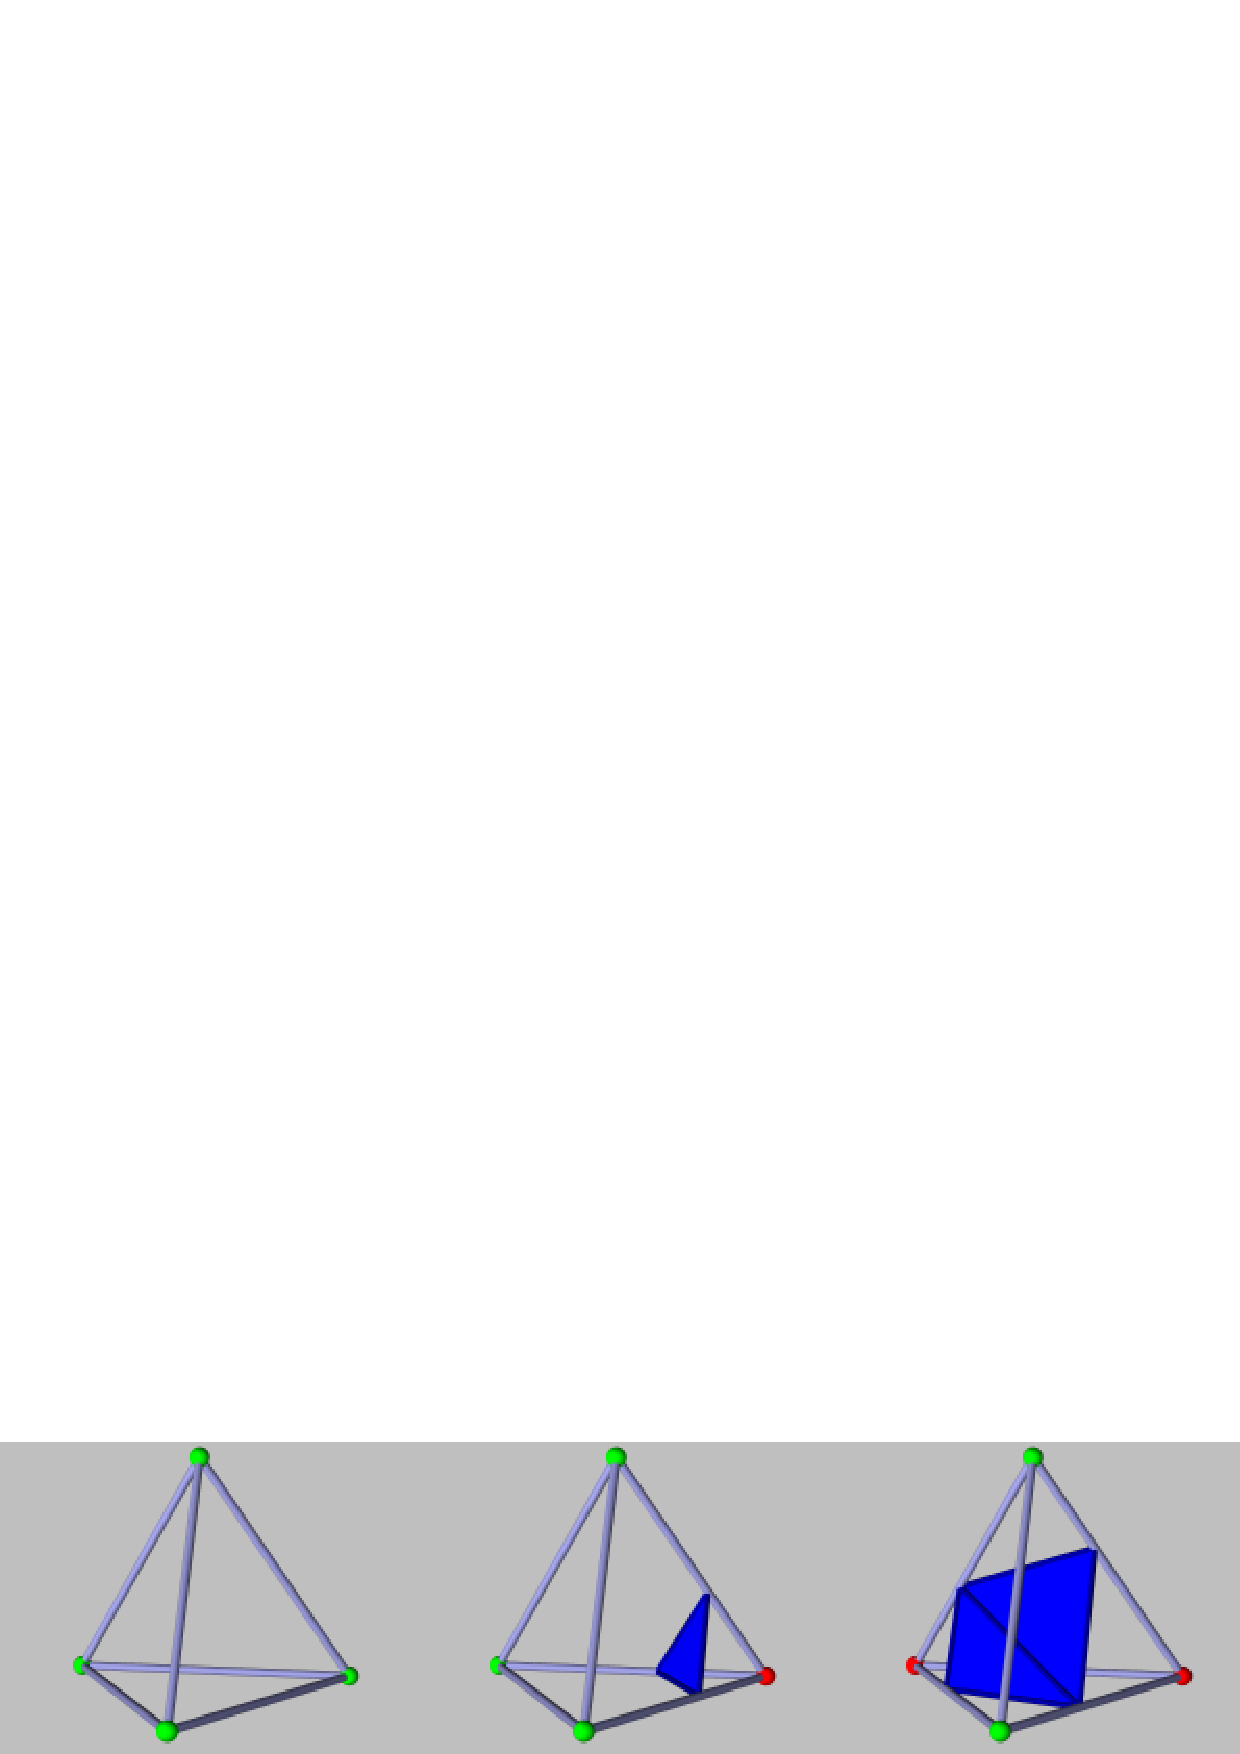
\includegraphics[width=\textwidth]{Skin_surface_3/marching}
\end{center}
\end{ccTexOnly}
\caption{Cases of the marching tetrahedra algorithm.
\label{SkinSurface3-fig-marching}}
\begin{ccHtmlOnly}
<CENTER>
<img border=0 src="./marching.png" align=center
alt="Cases of the marching tetrahedra algorithm.">
</CENTER>
\end{ccHtmlOnly}
\end{figure}

Our implementation takes four arguments: the input triangulation, the
output polyhedron, a traits class and an observer class.  The
algorithm is performed on the triangulation and stored in the
polyhedron. The \ccc{CGAL::Polyhedron_incremental_builder_3} is used for
constructing the polyhedron.

The traits class defines a single predicate and a construction. First
it is able to test whether a vertex of the triangulation lies inside
or outside the surface and it is able to return an intersection point
of the surface with an edge of the triangulation whose vertices lie on
opposite sides of the surface. For skin surfaces the intersection
point is unique.

The observer class implements two functions that are called after the
construction of a vertex and a facet of the polyhedron. After
insertion of a vertex in the polyhedron a function is called with the
vertex of the polyhedron and the corresponding edge of the
triangulation. Similarly, after insertion of a facet in the polyhedron
a function is called with the facet of the polyhedron and the
corresponding cell of the triangulation. Using these two functions it
is possible to construct a reference from simplices of the mesh to the
corresponding simplices of the triangulation.

Both the traits class and the observer class make this algorithm highly
flexible.
\subsection{Modifications to the mesh}
One algorithm is implemented to enhance the coarse mesh. It subdivides
the skin surface into smaller triangles and projects the new vertices
onto the mesh.
\section{Software Design}
NGHK: Back references
\section{Example programs}
The package contains wrapper function that constructs the coarse mesh
from an iterator range of weighted points.
\ccIncludeExampleCode{Skin_surface_3/skin_surface_simple.C}

% EOF


